% This must be in the first 5 lines to tell arXiv to use pdfLaTeX, which is strongly recommended.
\pdfoutput=1
% In particular, the hyperref package requires pdfLaTeX in order to break URLs across lines.

\documentclass[11pt]{article}

% Change "review" to "final" to generate the final (sometimes called camera-ready) version.
% Change to "preprint" to generate a non-anonymous version with page numbers.
\usepackage[final]{acl}
% \usepackage{natbib}

% Standard package includes
\usepackage{times}
\usepackage{latexsym}

% For proper rendering and hyphenation of words containing Latin characters (including in bib files)
\usepackage[T1]{fontenc}
% For Vietnamese characters
% \usepackage[T5]{fontenc}
% See https://www.latex-project.org/help/documentation/encguide.pdf for other character sets

% This assumes your files are encoded as UTF8
\usepackage[utf8]{inputenc}

% This is not strictly necessary, and may be commented out,
% but it will improve the layout of the manuscript,
% and will typically save some space.
\usepackage{microtype}

% This is also not strictly necessary, and may be commented out.
% However, it will improve the aesthetics of text in
% the typewriter font.
\usepackage{inconsolata}

%Including images in your LaTeX document requires adding
%additional package(s)
\usepackage{graphicx}
\usepackage{minted}
\usepackage{soul}
\usepackage{tabularray}
\usepackage{enumitem}
\setlist{nosep}

\UseTblrLibrary{booktabs}
\newmintinline[code]{html}{}
\DeclareRobustCommand{\note}[1]{{\sethlcolor{orange!30!white}\hl{#1}}}


\newcommand{\cA}{\mathcal{A}}
\newcommand{\cC}{\mathcal{C}}
\newcommand{\cP}{\mathcal{P}}
\newcommand{\bosun}[1]{\textcolor{orange}{{[bosun: #1]}}}
\newcommand{\amirali}[1]{\textcolor{blue}{{[amirali: #1]}}}
\newcommand{\jing}[1]{\textcolor{purple}{{[Jing: #1]}}}

\title{ Prompting is Not All You Need! Evaluating LLM Agent Simulation Methodologies with Real-World Online Customer Behavior Data}

% Author information can be set in various styles:
% For several authors from the same institution:
% \author{Author 1 \and ... \and Author n \\
%         Address line \\ ... \\ Address line}
% if the names do not fit well on one line use
%         Author 1 \\ {\bf Author 2} \\ ... \\ {\bf Author n} \\
% For authors from different institutions:
% \author{Author 1 \\ Address line \\  ... \\ Address line
%         \And  ... \And
%         Author n \\ Address line \\ ... \\ Address line}
% To start a separate ``row'' of authors use \AND, as in
% \author{Author 1 \\ Address line \\  ... \\ Address line
%         \AND
%         Author 2 \\ Address line \\ ... \\ Address line \And
%         Author 3 \\ Address line \\ ... \\ Address line}
\author{
  \textbf{Yuxuan Lu\textsuperscript{1,2}},
  \textbf{Jing Huang\textsuperscript{1}},
  \textbf{Yan Han\textsuperscript{1}},
  \textbf{Bingsheng Yao\textsuperscript{2}},
  \textbf{Sisong Bei\textsuperscript{1}},
\\
  \textbf{Jiri Gesi\textsuperscript{1}},
  \textbf{Yaochen Xie\textsuperscript{1}},
  \textbf{Zheshen (Jessie) Wang\textsuperscript{1}},
  \textbf{Qi He\textsuperscript{1}},
  \textbf{Dakuo Wang\textsuperscript{1,2}},
\\
\\
  \textsuperscript{1}Amazon.com, Inc.,
  \textsuperscript{2}Northeastern University
\\
  \small{
    \textbf{Correspondence:} \href{mailto:lu.yuxuan@northeastern.edu}{lu.yuxuan@northeastern.edu},
    \href{mailto:d.wang@northeastern.edu}{d.wang@northeastern.edu}
  }
}


%\author{
%  \textbf{First Author\textsuperscript{1}},
%  \textbf{Second Author\textsuperscript{1,2}},
%  \textbf{Third T. Author\textsuperscript{1}},
%  \textbf{Fourth Author\textsuperscript{1}},
%\\
%  \textbf{Fifth Author\textsuperscript{1,2}},
%  \textbf{Sixth Author\textsuperscript{1}},
%  \textbf{Seventh Author\textsuperscript{1}},
%  \textbf{Eighth Author \textsuperscript{1,2,3,4}},
%\\
%  \textbf{Ninth Author\textsuperscript{1}},
%  \textbf{Tenth Author\textsuperscript{1}},
%  \textbf{Eleventh E. Author\textsuperscript{1,2,3,4,5}},
%  \textbf{Twelfth Author\textsuperscript{1}},
%\\
%  \textbf{Thirteenth Author\textsuperscript{3}},
%  \textbf{Fourteenth F. Author\textsuperscript{2,4}},
%  \textbf{Fifteenth Author\textsuperscript{1}},
%  \textbf{Sixteenth Author\textsuperscript{1}},
%\\
%  \textbf{Seventeenth S. Author\textsuperscript{4,5}},
%  \textbf{Eighteenth Author\textsuperscript{3,4}},
%  \textbf{Nineteenth N. Author\textsuperscript{2,5}},
%  \textbf{Twentieth Author\textsuperscript{1}}
%\\
%\\
%  \textsuperscript{1}Affiliation 1,
%  \textsuperscript{2}Affiliation 2,
%  \textsuperscript{3}Affiliation 3,
%  \textsuperscript{4}Affiliation 4,
%  \textsuperscript{5}Affiliation 5
%\\
%  \small{
%    \textbf{Correspondence:} \href{mailto:email@domain}{email@domain}
%  }
%}

% \linespread{2}
\begin{document}

\maketitle
\begin{abstract}
Recent research shows that LLMs can simulate ``believable'' human behaviors to power LLM agents via prompt-only methods. 
In this work, we focus on evaluating LLM's objective ``accuracy'' rather than the subjective ``believability'' in simulating human behavior, leveraging a large-scale, real-world dataset collected from customers' online shopping actions. 
We present the first comprehensive evaluation of state-of-the-art LLMs (e.g., DeepSeek-R1, Llama, and Claude) on the task of web shopping action generation.
Our results show that out-of-the-box LLM-generated actions are often misaligned with actual human behavior, whereas fine-tuning LLMs on real-world behavioral data substantially improves their ability to generate accurate actions compared to prompt-only methods.
Furthermore, incorporating synthesized reasonings into model training leads to additional performance gains, demonstrating the value of explicit rationale in behavior modeling.
This work evaluates state-of-the-art LLMs in behavior simulation and provides actionable insights into how real-world action data can enhance the fidelity of LLM agents.
\end{abstract}

\section{Introduction}

Recent advances in large language models (LLMs) have enabled the simulation of ``believable'' human behavior across a range of applications, including web navigation actions~\cite{gurRealWorldWebAgentPlanning2023, zhouWebArenaRealisticWeb2024}, social interaction behaviors~\cite{parkGenerativeAgentsInteractive2023}, interpersonal trust behaviors~\cite{xieCanLargeLanguage2024}, and user interface interactions~\cite{taebAXNavReplayingAccessibility2024}. 
These developments have sparked growing interest in using LLMs to power agentic systems that emulate human behaviors (\textbf{LLM Agent})~\cite{chenDesignGuidelineRPA2025}. 
Despite these successes, current evaluations~\cite{parkGenerativeAgentsInteractive2023} primarily emphasize subjective measures of ``\textbf{believability}'' (``how much people feel it is like a human'') instead of the objective ``\textbf{accuracy}'' (``how much it acts like a human'').
The most relevant works that measure the objective model accuracy focus only on the final outcome of a task (e.g., purchasing the final product or not~\cite{yaoReActSynergizingReasoning2023},  or ultimately trusting the partner or not~\cite{xieCanLargeLanguage2024}), rather than rigorously evaluating whether the generated sequence of actions mirrors authentic human behavior or not.
Consequently, the field currently lacks a robust and quantitative understanding for assessing LLMs at the process-centric, action-level simulation of human behaviors.


\begin{figure}[t]
    \centering
    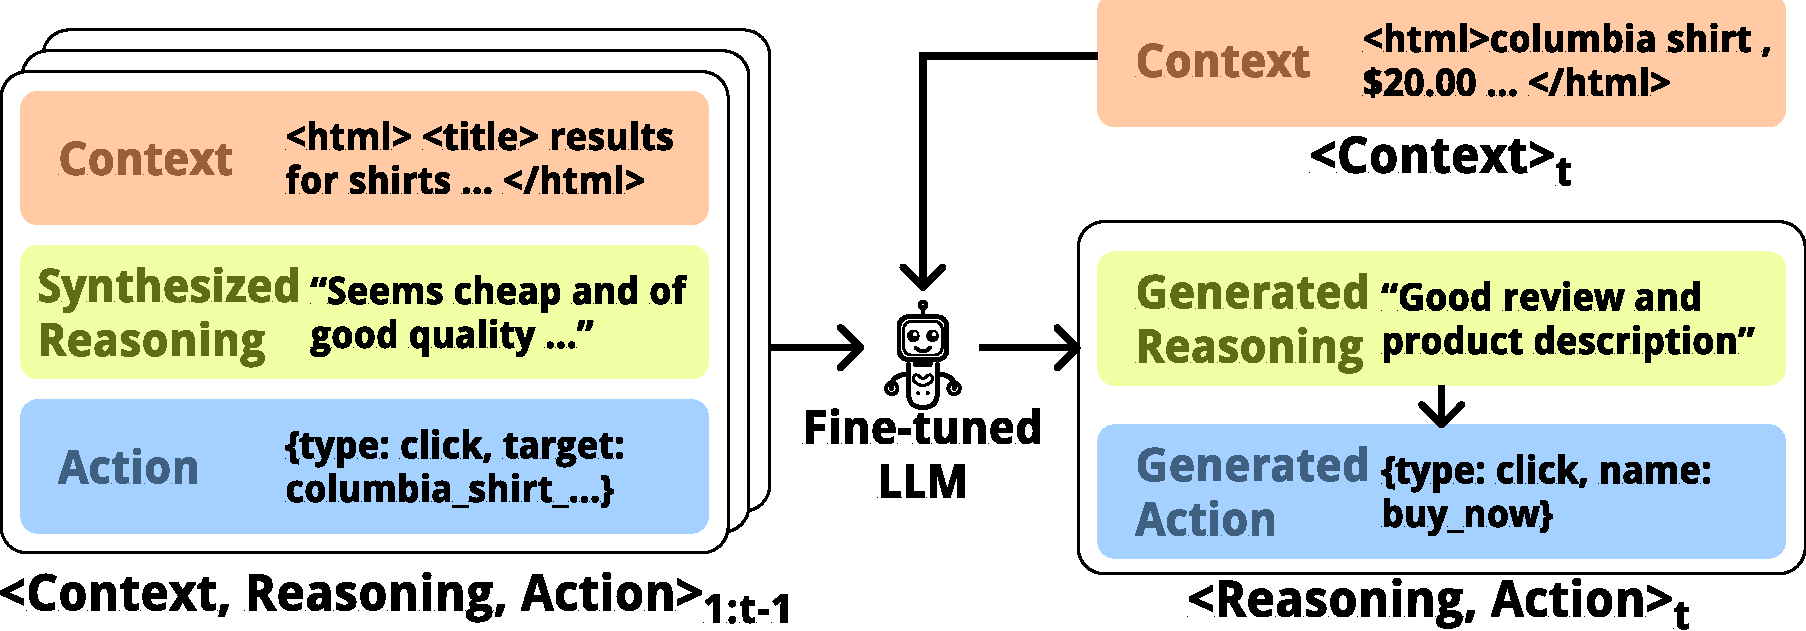
\includegraphics[width=\linewidth]{figures/teaser.pdf}
\caption{Overview of the web action generation task. The model takes the currently observed \textbf{<context>$_{t}$} and a sequence of previous \textbf{<context, reasoning, action>$_{1:t-1}$} as input, and generates the next \textbf{<reasoning, action>$_{t}$} as output. Because the real-world human behavior dataset does not have groundtruth reasoning, we generate \textbf{synthesized reasoning trace} to complement the <context, action> pair. }
    \label{fig:model-arch}
    \vspace{-\baselineskip}
\end{figure}

In this paper, we focus specifically on the \textbf{human behavior simulation} task, which is to generate the next most likely user action based on the current observation and the history of past actions. For instance, in an online shopping scenario, the model observes the current webpage context (e.g., a product list) and the user’s action history (e.g., previous clicks or queries), and generates the next plausible action a human would take.
Real human users often implicitly form reasoning traces behind their action behaviors~\cite{caoThinkingFastSlow2023}. 


To bridge this gap, our work provides the first systematic evaluation of SOTA LLMs' accuracy in process-centric, action-level behavior simulation tasks.
We leverage a large-scale, real-world dataset consisting of 31,865 user sessions of 3,526 users from an online shopping platform.
Each session (Figure~\ref{fig:model-arch}) comprises a series of timestamp-aligned <context, action> pairs, where the context reflects the webpage observed by the user (e.g., product views, filter states), and the action denotes user inputs such as clicks, searches, or session termination actions.
In total, the dataset has 230,965 user actions, and the final outcomes of the sessions include 4,432 purchase actions and 27,433 session termination actions.
This dataset enables us to rigorously evaluate how accurately various LLMs can generate human-like behaviors at the action level.
We evaluate different models on the next action generation task, benchmarking both the accuracy of generated actions throughout the session and the F1 score for final action generation, following protocols similar to existing work on modeling online shopping behavior.

Beyond evaluation, our dataset uniquely positions us to\textbf{ fine-tune} LLMs to enhance their accuracy in behavior simulation tasks. 
While prior work has primarily relied on prompt-based approaches, we show that model adaptation through fine-tuning leads to significantly better accuracy in action generation and session outcome prediction.
Furthermore, drawing inspiration from reasoning-augmented modeling \cite{deepseek-aiDeepSeekR1IncentivizingReasoning2025}, we hypothesize that exposing models to intermediate reasoning traces--even if synthetically generated--can enhance their ability to simulate human behavior.
To test this hypothesis, we augment our dataset with synthesized reasonings from action traces using Claude 3.5 Sonnet and fine-tune models using this augmented data (\texttt{<context, action, reasoning>} triplets) to learn how to generate not only accurate actions but also the underlying reasoning.
Our results show that this reasoning-augmented fine-tuning further boosts model performance, highlighting the importance of modeling not just what humans do, but also why they do it.

In summary, this paper has two contributions:

\begin{itemize}
    \item We provide the \textbf{first quantitative and process-centric evaluation} of LLMs to simulate human web action behaviors using real-world data from an online shopping context.
    
    \item Through our evaluation, we empirically demonstrate that \textbf{fine-tuning LLMs with synthesized reasoning significantly improves model's performance}, highlighting the value of incorporating explicit reasoning to improve the fidelity of LLM agent applications for role-playing or behavior simulation .
\end{itemize}
% To summarize, our contributions are as follows:  
% \begin{enumerate}  
% \item We present the first \textbf{quantitative evaluation} of state-of-the-art prompt-based LLMs in simulating human behavior, using a large-scale dataset from a real-world online shopping scenario.  
% \item We demonstrate that \textbf{fine-tuning with synthesized reasoning trace} significantly improves action generation accuracy, laying the foundation for future research in role-playing agents and digital twin simulations.  
% \end{enumerate}


% para1:
% Recent research work on llm agent system are promising -- because llm can simulate believable human behavior
% llm models have been proven to be able to simulate web browsing behavior -- (webagent webnarena ..) -- social interaction behavior --  trust behavior -- user interact behavuir (uxnav).
% (
% mention one of the two keywords in the title, ...
% however the evaluation of the llm models in these various human behavior works have been missing, as they only evaluate the ``believibility'' of the model .
% without real-world behavioral data based evaluation ,we are unable to benchmark these models in particular on their capability of simulating real human behavior. 
% although task-oriented agent can do well, we are unable to know their capability in simulation of human behavior.
% in order to evaluate -- we need real-world data -- evaluation task for ...
% [or]
% all human behavior simulation  system used prompt-based approach rather than fine-tuning on real behavior data
% )


% para2: what is the task.
% specifically, human behavior simulation task -- use old behavior to generate next behavior, based on the current observation -- for example, in park sim paper -- the core functionality is to generate the reflection/reasoning/plan based on the observation of the outside world -- and generate the next action based on the internal reflection.
% the current evaluation focus on either final outcome (park 1000), distribution, believility.
% action-leval decision making should not only align with the final outcome 

% para3:
% in this work, we have the privilege of ... a 30k user session data from x user and x action with x purchase and x terminate  .. in the online shopping scenario 
% [explain dataset based on figure 1]
% as shown in figure 1, the dataset consists of a sequence (t=1 -- n) of context and action pair. the context is ..
%  the action is one of the ...
% this dataset enable us to systematically evaluate the accuracy ...
% [don't mention fine-tune]
% [one -sentence summary of the construction of test dataset]

% para4:
% In addition to evaluation, we can also use this dataset for fine-tuning to improve the model's performance in simulation of human behavior in the online shopping scenario.
% this is also unique .. in the human simulation task -- other only used a prompting strategy.
% further, inspired by recent reasoning work (deepseek r1?),  the reasoning/ reasoning can further improve model's performance. however, this is not directly available in our dataset -- thus we augment the adtaset with claude -- synthesize a reasoning at each step of human behavior trace.
% then, use the triplet <context, action, reasoning>, we finetune.
% our result demonstrated ....

% par 5
% in summary, 1 use dataset to evaluate sota model prompt-based only behavior simulation ability
% 2) we finetune .. reasoning works. enabled future role-play and digital twin agent development 






% Recent research has highlighted an exciting trend that large language models (LLMs) can simulate ``believable'' human behaviors thus enabling promising agentic AI applications such as LLM Agents~\cite{chenDesignGuidelineRPA2025}, Web Agents~\cite{gurRealWorldWebAgentPlanning2023,iongOpenWebAgentOpenToolkit2024}, and GUI Agents~\cite{zhangAPIAgentsVs2025}. 
% Prior work has explored two key aspects of this capability. 
% First, some studies focus solely on the qualitative believability of LLM-generated behaviors, such as agents autonomously interacting in a simulated town environment and exhibiting human-like social interactions \cite{parkGenerativeAgentsInteractive2023}.
% Second, other studies evaluate LLMs based on their ability to replicate the final outcomes of controlled social science studies, such as survey results, without assessing whether the decision-making process aligns with real human behavior \cite{parkGenerativeAgentSimulations2024}. 
% However, in the real world, human behavior consists of a series of actions leading to a final outcome, and an accurate simulation should align not only with the end result but also with the action-level decision-making process.

% While existing literature has demonstrated the potential of LLMs in in-context learning (ICL) settings through qualitative evaluation studies, we have identified two key research gaps in those studies.
% To begin with, in-context learning may be inferior to fine-tuning methods in human behavior simulation, as a similar trend has been observed in other tasks and domains \cite{xuMentalLLMLeveragingLarge2023, luHumanStillWins2023}.
% Additionally, most prior studies primarily focus on assessing the \textbf{believability} of model-generated behaviors rather than their \textbf{action-level accuracy}, largely due to the lack of real-world human behavioral data for quantitative evaluation. 
% However, believability alone does not confirm that LLMs can truly model human behavior—it only shows that their outputs appear plausible.
% Without quantitative accuracy measures, there is no proof that the model’s simulation aligns with real human behavior.
% Thus, we still do not know whether existing LLM-based Agents can truly model human decision-making processes or if they merely generate superficially plausible behaviors.
% % Without a rigorous, data-driven evaluation framework, the effectiveness of these models in faithfully simulating real-world human behavior remains uncertain.

% In this work, we have the privilege of accessing a large-scale, real-world human behavioral dataset in the online shopping domain. 
% Shopping represents a common human activity that involves complex decision-making processes influenced by various factors such as context and prior experiences \cite{karimiEffectPriorKnowledge2015}. 
% This dataset enables us to fine-tune LLMs for human behavior simulation in the shopping domain and systematically evaluate their accuracy by comparing the simulated LLM agent behaviors with real-world human behavior.


% In this work, we focus on improving the accuracy of LLM-based human behavior simulation by fine-tuning an open-source LLM on a large-scale dataset of human behavior.
% To enrich this dataset, we introduce a synthesized reasoning for each action, providing additional context that enhances the model’s understanding of the human decision-making process.
% We evaluate our approach using a subset of our dataset and compare its performance against strong baseline LLMs in ICL settings.
% As illustrated in Figure \ref{fig:model-arch}, our fine-tuned model processes enriched behavioral inputs to generate more accurate action predictions.
% Our results demonstrate that fine-tuning enriched behavioral data significantly improves prediction accuracy by \note{2.38$\times$}, highlighting the crucial role of synthesized reasoning trace in achieving realistic human behavior simulation.

% To summarize, our contributions are as follows:
% \begin{enumerate}
% \item To the best of our knowledge, we present the first \textbf{quantitative evaluation} of current LLM Agent systems’ performance using real-world human behavioral data.
% \item We provide \textbf{empirical evidence} that fine-tuning LLMs with synthesized reasoning trace and real-world behavioral data leads to superior performance compared to out-of-the-box LLMs.
% \end{enumerate}

\section{Related Works}
\subsection{Simulation of Human Behavior with LLM }


% Emerging LLM agent research suggests LLM is capable of simulating believable human behaviors. 
The core function of the emerging LLM agent systems is their capability of generating human behaviors, in which a model takes a static user persona (e.g., preferences, demographics, or shopping habits), and the session data (e.g., a sequence of actions) as input to generate the next user action.
Such systems have been extensively utilized and tested to simulate human behavior in a variety of scenarios.
\citet{parkGenerativeAgentsInteractive2023} simulated social behavior using generative agents in a virtual town, producing ``believable'' interactions.  
\citet{xieCanLargeLanguage2024} studied LLM agents in Trust Games to assess their ability to model human trust behavior.  
\citet{parkGenerativeAgentSimulations2024} used LLMs to simulate responses from 1,052 individuals in a social science survey.  
To simulate UI interaction, \citet{luUXAgentLLMAgentBased2025} proposed UX\-Agent, enabling LLMs to operate within web environments for simulated usability testing.
Collectively, these studies underscore the growing potential of LLM-driven simulations to model and simulate complex, interpretable human behaviors.


However, the evaluation of these works remains limited in scope. Some focus on the subjective believability of process-centric action traces. 
For instance, \citet{luUXAgentLLMAgentBased2025} conducted qualitative interviews to assess participants' perceptions of the realism of their UXAgent system.
Similarly, \citet{parkGenerativeAgentsInteractive2023} proposed an evaluation framework that identified emergent social behaviors among generative agents.
On the other hand, works that pursue objective evaluation often do so in a single-shot, outcome-centric manner.
\citet{zhouWebArenaRealisticWeb2024} introduced WebArena, a controlled environment for benchmarking web agents based on task completion rates. ReAct \cite{yaoReActSynergizingReasoning2023} measured success rates in simulation environments, overlooking the accuracy of model mimicing step-by-step human behavior.
To date, no prior work has focused on \textbf{objectively evaluating model-generated  action traces}--that is, assessing whether a model's sequence of decisions faithfully aligns with human behavior at each step.

\subsection{Reasoning in Human Behavior Simulation}  

Building on the chain-of-thought prompting strategy \cite{weiChainofThoughtPromptingElicits2023}, numerous studies have incorporated reasoning mechanisms into human behavior simulation.  
\citet{parkGenerativeAgentsInteractive2023} pioneered agents equipped with reflection modules that synthesize memory and social context to support introspective decision-making. 
ReAct \cite{yaoReActSynergizingReasoning2023} prompted models to generate reasoning traces and actions separately, improving task success rates in online shopping and gaming environments.  
\citet{gurRealWorldWebAgentPlanning2023} proposed WebAgent, which uses a dedicated reasoning model to plan sub-steps in web browsing tasks, enhancing control and planning in real-world browser simulations.  
Beyond single-agent reasoning, systems such as ChatDev \cite{qianChatDevCommunicativeAgents2024} and RepoAgent \cite{luoRepoAgentLLMPoweredOpenSource2024} adopt multi-agent setups, where agents with specialized roles (e.g., programmers, testers) engage in collaborative dialogues via structured prompts. These communicative exchanges support more robust collective reasoning, demonstrating how coordination between agents can improve the quality of generated reasoning traces.

However, the aforementioned works incorporate reasoning using prompt-only approaches for the action generation task. Whether reasoning can improve performance in \textit{fine-tuning} settings remains an open question.
Although datasets for reasoning behind model actions exist (e.g., for conversational agents~\citep{dongreReSpActHarmonizingReasoning2025}), there is currently no ready-to-use dataset specifically designed for human behavior simulation that includes both human actions and the corresponding reasoning behind those actions.
To address a similar cold-start problem in reinforcement learning, \citet{deepseek-aiDeepSeekR1IncentivizingReasoning2025} constructed a small-scale dataset of long reasoning traces by synthesizing examples through few-shot prompting, followed by reflection and verification. Inspired by their methodology, we apply a similar strategy to synthesize reasoning traces in the online shopping domain. This enables us to investigate whether integrating reasoning into fine-tuning can enhance a model's ability to accurately simulate human behavior.


\section{Method}

\subsection{Task Definition}  

In this section, we formally define the proposed human behavior simulation task: in the online shopping scenario,  a shopping session is represented as a sequence of user actions $a_{1 \dots t \dots N}$, always starting with a \texttt{search action} and concluding with either a \texttt{product purchase action} or a \texttt{termination action} (i.e., the user closing the browser window).  

At each time step \( t \), the model is tasked with generating both \textbf{the reasoning \( r_t \)} and \textbf{the  action \( a_t \)}. The model input includes the current context \( c_t \) (what the user currently observes), a sequence of previous contexts (what the user has observed) \( c_{1 \dots t-1} \), a sequence of previous actions \( a_{1 \dots t-1} \) (what the user has done), and the corresponding synthetic reasoning trace \( r_{1 \dots t-1} \) (why the user had that action) within the same session. Formally, the model learns a function \( f \) such that:  
\[
    f(c_{1 \dots t}, a_{1 \dots t-1}, r_{1 \dots t-1}) = r_t, a_t
\]

% To ensure contextual plausibility, all user actions within a session—such as clicks—must be performed on items or links that were previously displayed to the user.
% This constraint prevents the model from generating unrealistic actions and ensures that its predictions remain grounded in the user's browsing history.

\paragraph{Observation Context}

% The Context, also referred to as the ``observation space'' of the web environment, represents the information available on a web page, including textual content, metadata, visual elements, and structural data. This context is designed to capture how users observe web pages, enabling an agent to process relevant information for navigation, retrieval, and interaction.

% Following recent work \cite{luUXAgentLLMAgentBased2025}, we adopt a structured representation of the web page using a \textbf{simplified HTML format}, which preserves key structural elements while filtering out irrelevant details such as scripts and styling information.
% To facilitate precise action execution, each interactable element (such as links, buttons, and input fields) is assigned a unique hierarchical ``name'' that incorporates parent-child relationships within the webpage. These names serve as identifiers in the action space, ensuring that the agent can correctly reference and interact with specific elements. A description definition of our context design can be found in Appendix \ref{sec:context}.

The \textbf{Context} (or ``observation space'') of the web agent encompasses all available information on a webpage, including textual content, metadata, visual elements, and structural data. This context is designed to reflect how a human perceives and interprets a webpage, allowing the agent to process relevant features and perform tasks such as navigation, information retrieval, and interaction with page elements.  

Previous research has explored various approaches to defining the context. Some methods rely on manually structured information parsing \cite{yaoWebShopScalableRealWorld2022}, while others utilize raw HTML representations \cite{gurRealWorldWebAgentPlanning2023} or accessibility tree embeddings \cite{zhouWebArenaRealisticWeb2024}. However, both approaches have notable limitations: manually structured information parsing requires significant human effort to develop parsing rules \cite{yaoWebShopScalableRealWorld2022}, while raw HTML representations often contain extraneous information (e.g., CSS) that is not directly observable to human users, which may bias the LLM performance.  

To ensure the adaptability to unseen websites, we define and implement a \textbf{simplified HTML} format as our context representation. This format removes non-relevant elements such as scripts, CSS, and purely visual components while preserving essential structural information. Using simplified HTML offers several advantages over custom formats or markdown-based representations: (1) important structural elements, such as lists and tables, remain intact, and (2) LLMs are already familiar with the HTML format, eliminating the need to redefine common elements like `button' and `input'.

The LLM agent needs to refer to specific elements within the HTML, such as identifying the exact button it intends to click. Since there is no built-in method to uniquely identify HTML elements, prior work has proposed approaches like assigning sequential IDs to elements \cite{kohVisualWebArenaEvaluatingMultimodal2024} or manually defining descriptive names for elements, such as \code{searchbox} \cite{yaoWebShopScalableRealWorld2022}. Following prior work \cite{luUXAgentLLMAgentBased2025}, we assign a unique hierarchical \textit{name} in natural language to each interactable element, including links, buttons, and input fields. This name is constructed by incorporating the names of all parent nodes. For instance, if a \code{<a>} tag named \code{view_product} resides within a \code{<div>} named \code{columbia_shirt}, the resulting hierarchical name will be \code{columbia_shirt.view_product}.

\paragraph{Reasoning}

Reasoning trace refers to a natural language description that articulates the reasoning and explanation behind an action.
% By also generating reasonings for each action, the fine-tuned model not only improves transparency in decision-making but also makes its generations more interpretable.
For example, if the context is a search results page displaying a list of clothes, and the generated action is clicking on the \code{"4 stars and up"} product review filter, the generated reasoning might be: \textit{``I want to find a comfortable piece of clothing, so I’m looking for options with high ratings.''}
In our domain, the reasoning trace is missing from any real-world online shopping data, so we use LLM to synthesize it (Section~\ref{sec:data-synthesize}).
The generated reasoning provides insight into the model's thinking process, enhancing the transparency of the model's generations.

\paragraph{Action}
Previous research has explored various approaches to defining action spaces, including task-specific semantic actions such as ``searching'', ``adding items to a cart'', and ``making purchases'' \cite{yaoWebShopScalableRealWorld2022}, as well as browser-level interactions like \texttt{typing} and \texttt{clicking} \cite{luUXAgentLLMAgentBased2025}. 

To ensure the adaptability of our framework beyond online shopping tasks, we define the action space at the level of \textbf{raw browser actions}, rather than at the level of task-specific semantics.
The action space of our model consists of three fundamental browser operations: \code{click}, \code{type_and_submit}, and \code{terminate}.
This abstraction allows the system to generalize across different environments while maintaining task flexibility.
\label{sec:action-definition}

To comprehensively evaluate the performance of our model, we also evaluate the \textbf{final outcomes} of the shopping session.
The final outcomes consist of either a purchase action or a termination action.
Since the final outcome is always the last action in a session, it marks the conclusion of the user’s shopping journey.
This evaluation setup allows for a more detailed analysis of how accurately the model can generate both process-centric action-level behaviors and the final shopping outcomes.

\subsection{Synthesized Reasoning Trace}
\label{sec:data-synthesize}
Reasoning traces are crucial for understanding users' action choices but are difficult to collect; thus, they are often not available in behavioral datasets.
We employ a reasoning synthesis pipeline to generate them using an LLM.
To guide the reasoning generation process, we provide the LLM with the observation context and the corresponding action.
Additionally, we record a real human customer's think-aloud shopping sessions as in-context learning examples.

The LLM is then prompted to generate a free-text reasoning explaining the user's decision.
This approach ensures that the synthetic reasoning traces are both coherent with the action and reflective of human reasoning.
By bridging the gap between raw behavioral data and the reasoning processes, our method enhances the explainability of the model.

\subsection{Model Architecture}

To incorporate these enriched action traces, we build on existing pre-trained LLMs as our base models.
The input to the model consists of two components: \textbf{(1) a sequence of historical contexts} (what the user observed), and \textbf{(2) the corresponding actions and generated reasoning trace} (what the user did and why). The model is trained to generate the next reasoning and action, enabling it to simulate human behavior with greater fidelity.

During the \textbf{training stage}, the model receives the full sequence of a user session—including context, synthetic reasoning, and action—as a single concatenated input. 
The training objective is to minimize the next-token prediction loss for the reasoning and action tokens, while the loss for the context tokens is masked out. 
Subsequently, in the \textbf{evaluation stage}, the model is provided with historical context and past reasoning traces and actions. The model first generates the reasoning for the next action; then, based on the generated reasoning, it generates the next action.

\section{Experiments}
\subsection{Dataset Construction}

Our training dataset was constructed using data from one of the largest e-commerce platforms globally.
The dataset contains 31,865 user sessions from 3,526 users in the online shopping scenario, comprising  230,965 user actions.
The session's final outcome includes 4,432 purchase actions and 27,433 session termination actions.
We leveraged our data synthesis pipeline detailed in Section \ref{sec:data-synthesize} to generate the synthetic reasoning for each action based on the context
using Claude-3.5-Sonnet.

% \jing{No need to explain this part because it is confusing to what have been described above. Recommend removing this paragraph.}
% Due to the noisy nature of real-world behavioral logs, many sessions in our raw dataset contain actions that fall outside our defined action space. For example, users may open product pages directly from external sources such as search engines, advertisements, or shared links.
% These actions are considered invalid in our setting because the required context—what was displayed to the user at the time—is unavailable, making it impossible for the model to reason about or replicate the behavior.
% To ensure consistency and validity in training and evaluation, we remove all sessions containing such invalid actions through a rigorous data-cleaning process.

We extracted pairs of user actions and contextual information from the cleaned data. These raw logs were then structured into the standardized format defined in Section \ref{sec:action-definition}.

\subsection{Evaluation and Metrics}

\paragraph{Evaluation Dataset}  

We used a subset of the dataset that was not used during training as the test set, ensuring that no user sessions in the test set were seen by the model during fine-tuning.
To create test cases, we took the second and all subsequent actions within each session, excluding the first action, since it lacks any preceding context.
For each test case, the model was provided with the historical context, along with all previous actions and corresponding synthetic reasoning traces in the same session.
The model is \textbf{first tasked with predicting the next reasoning, and then, based on the reasoning it generated}, it produces the corresponding action.
% and tasked with predicting both the next reasoning and the corresponding action.   

This setup allows us to evaluate the model's performance in a sequential reasoning setting, closely mirroring how real users behave during the session. This process resulted in a total of 357 sessions with 932 test cases.

\paragraph{Prompt-Only Baseline}
To compare against our fine-tuned models, we evaluated a set of strong instruction-tuned LLMs under the in-context learning (ICL) setting (a.k.a., prompt-based setting). Specifically, we used several variants of Claude, LLaMA, and Mistral as representatives for general-purpose pre-trained LLMs, along with DeepSeek-R1 as a representative for reasoning LLMs.

In this setup, each model was provided with the historical context and previous user actions from the session, and prompted to generate both the next reasoning and the next action.
The generated actions were used to compute macro accuracy for evaluation. 
These baselines reflect the commonly adopted approach of using powerful LLMs without domain-specific fine-tuning, allowing us to directly assess the impact of fine-tuning on realistic human behavior simulation.



\begin{table}[t]
\centering
\begin{booktabs}{
  colspec = {X[l]cc},
  cells={m},
  cell{10,12,14}{1}={r,font=\itshape},
}
\toprule
Model                         & { Action Gen. \\ (Acc.) }& {Outcome \\ (F1)} \\
\midrule 
{Llama 3.1 70B}       & 8.19\%              & 12.69\%            \\
{Claude 3.5 Sonnet}& 9.72\%            & 15.91\%            \\
{Claude 3.7 Sonnet}   & 9.34\%              & 12.81\%            \\
{DeepSeek-R1}         & \textbf{11.86\%}             & \textbf{20.01\%}            \\
Qwen2.5-7B           & 4.25\%              & 11.94\%      \\
Mistral-7B-v0.3      & 4.25\%              & 11.27\%      \\
Llama 3.2 3B         & 2.93\%              & 8.60\%       \\
\midrule
Qwen2.5-7B SFT                    & \textbf{17.26\% }            & 33.86\%            \\
w/o reasoning                 & 16.67\%             & 26.92\%            \\
Mistral-7Bv0.3 SFT               & 15.84\%             & 30.12\%            \\
w/o reasoning                 & 14.17\%             & 17.99\%            \\
Llama-3.2-3B SFT                  & 15.77\%             & \textbf{33.99\%}            \\
w/o reasoning                 & 9.31\%              & 4.73\%             \\
\bottomrule
\end{booktabs}
\caption{Model performance. The top four models are prompt-only, and the bottom three models are fine-tuned with or without synthesized reasoning traces. The table shows model accuracy in two tasks: the process-centric \textbf{action generation} task and the \textbf{outcome}-centric final purchase prediction task of the session. More models' performances are in the Appendix.}
\label{tab:results}
\end{table}

\paragraph{Evaluation Metrics}  
% \note{todo: elaborate on the task.}

We evaluate model performance across two key dimensions: \textbf{Next Action Generation} and \textbf{Session Outcome Classification}.

For \textbf{Next Action Generation}, we evaluate whether the model can accurately generate user actions during the process.
We use an \textit{\textbf{exact match accuracy}}, where a generation is considered correct only if the action type, action target (e.g., search box or product link), and action attribute (if applicable, such as search keyword) exactly match the ground truth. 
To avoid skewing the results toward longer sessions, we compute per-session accuracy first and then average across sessions, ensuring each session contributes equally to the final score.

To evaluate models' performance beyond human behavior simulation to shopping prediction, we introduce an additional task and metric focused on the \textbf{session final outcome }. 
The evaluation setting remains the same: the model is given the ground-truth session history up to the last step and tasked with generating the next (and final) action. 
Since the final action is always either a \code{click} action on the \code{buy now} button or a \code{terminate} action indicating closing the browser window, we evaluate the binary classification performance using the F1 score. 
This allows us to assess how well the model distinguishes between these two critical session outcomes (\texttt{buy} or \texttt{termination}).



\begin{figure*}[t]
    \centering
    \includegraphics[width=.7\linewidth]{figures/action_distribution_below_labels}
    \caption{Action categories of human groundtruth, and generated by prompt-based Claude and by our fine-tuned models.}
    \label{fig:action-distribution}
    \vspace{-\baselineskip}
\end{figure*}


\subsection{Experimental Setup}
We fine-tuned multiple language models to evaluate their performance on the action generation task. The models used in our experiments include:
\begin{itemize}
    \item \textbf{Fine-Tuned Models:} Different versions of Llama 3.2, Qwen 2.5, and Mistral.
    \item \textbf{Baseline Models:} Different versions of Claude, Llama, Mistral, and DeepSeep-R1.
\end{itemize}
All fine-tuned models were trained using the same dataset and pipeline to ensure a fair comparison. 

Model training was performed on a GPU cluster consisting of NVIDIA H200 GPUs, with each training job utilizing eight nodes, each equipped with eight GPUs, for a total of 64 GPUs, each with 140 GB of GPU memory.

We employed Fully Sharded Data Parallel \cite{zhaoPyTorchFSDPExperiences2023} for efficient training. All sequences were padded or truncated to a context length of 40k tokens. We used a per-device batch size of 1, resulting in a global batch size of 64. The learning rate was set to 2e-5 with a cosine scheduler for adaptive learning rate adjustment. Models were trained for 1 epoch. For example, training Mistral-7B-v0.3 with a 40k token context window in our setup requires approximately 130GB of GPU memory per GPU, which is the largest model we can train.



\begin{figure*}
    \centering
    \includegraphics[width=.8\linewidth]{figures/error_analysis.pdf}
    \caption{Error Type Analysis of different models.}
    \label{fig:error-analysis}
\end{figure*}


\subsection{Evaluation Results and Analysis}


% following xx we evaluate icl of ... deepseek best

% we fine-tuned ... qwen 7b best in our task -- in addition final outcome ..
Following previous works \cite{lutzWILBURAdaptiveInContext2024, dengMind2WebGeneralistAgent2023}, we evaluate the performance of prompt-based LLMs in simulating human behavior on shopping scenarios, with results presented in Table~\ref{tab:results}.
Our findings indicate that while state-of-the-art LLMs have demonstrated strong capabilities in various tasks and domains, their ability to accurately simulate human behaviors remains limited.
Compared to general instruction-tuned models, reasoning-focused DeepSeek-R1 achieved a higher accuracy of \textbf{11.86\%} in the action generation task, suggesting that incorporating reasoning mechanisms offers some advantage.
Similarly, for final outcome prediction, DeepSeek-R1 attained an F1 score of \textbf{20.01\%}, outperforming other baseline models.
These results highlight the challenges of human behavior simulation and suggest that reasoning models may provide incremental improvements, though significant gaps still remain.

We then fine-tuned LLaMA 3.2, Qwen 2.5, and Mistral using our training dataset. The results demonstrate that fine-tuning LLMs with action traces and synthesized reasoning traces significantly enhances performance. Qwen 2.5-7B achieved \textbf{17.26\%} accuracy in action generation, significantly surpassing DeepSeek-R1 by \textbf{5.4\%} {($p < 10^{-10}$, McNemar's test)}. Similarly, LLaMA 3.2-3B reached an F1 score of \textbf{33.99\%} on the final outcome prediction task, further confirming the effectiveness of fine-tuning.
{All fine-tuned models significantly outperformed their own ICL variants ($p < 10^{-5}$, McNemar's test).}
These findings underscore that incorporating domain-specific fine-tuning with synthesized reasoning traces leads to substantial improvements in the accuracy of human behavior simulation.

We also visualize the distribution of user actions across different models compared to real human behavior in Figure~\ref{fig:action-distribution}.
The fine-tuned models exhibit a distribution that more closely aligns with human action patterns, capturing a more natural balance between search, product clicks, and filter actions. In contrast, Claude 3.5 Sonnet and DeepSeek-R1 displays a noticeably higher purchase rate while conducting only a single search per session, diverging from actual user behavior. This misalignment suggests that fine-tuning not only improves accuracy but also helps models better replicate realistic shopping behaviors rather than over-prioritizing purchase actions.



\subsection{Ablation Study}  

To evaluate the impact of synthesized reasoning traces on the model's action generation capability, we conducted an ablation experiment.  In the \textit{``w/o reasoning''} settings, we removed the reasoning from the model input, and we trained and evaluated the model using only the context and action. This experiment helps us to learn whether learning from synthesized reasoning traces improves the model’s ability to generate user actions.



From Table~\ref{tab:results}, most models exhibited a significant drop in action generation accuracy when trained without reasoning traces, highlighting the importance of explicit reasoning in guiding predictions. A similar decline was observed in final outcome prediction, with F1 scores consistently decreasing across models.
For instance, Qwen2.5-7B achieved a \textbf{33.86\%} F1 score with reasoning traces but dropped to \textbf{26.92\%} without, demonstrating that reasoning traces play a crucial role in improving model performance.
These results confirm that incorporating synthesized reasoning traces enhances both action generation and final outcome modeling, reinforcing their value in fine-tuning for human behavior simulation.

\subsection{Error Analysis}

We analyze model behavior across different error types, comparing two ICL models, Claude, representing general-purpose chat models, and DeepSeek-R1, representing reasoning-augmented models, with a fine-tuned compact model, Qwen2.5–7B.
We focus on five distinct error types. \textbf{Didn’t terminate}, \textbf{didn’t click}, and \textbf{didn’t search} indicate cases where the model chose a different action instead of terminating, clicking, or searching, as the human user did. \textbf{Searched wrong keyword} refers to instances where the model performed a search like the user, but used a different (and incorrect) search query. \textbf{Clicked wrong button} captures cases where the model clicked, but on a different button than the one selected by the human user.
Illegal actions generated by models are excluded from this analysis.
Overall, Claude and DeepSeek-R1 exhibit very similar error profiles, suggesting that the reinforcement learning process used to incorporate reasoning introduces similar biases to those seen in standard chat-based ICL models.

A major shared failure mode of ICL models is their tendency to continue sessions even when human users would have terminated them by closing the browser window. This aligns with earlier findings that ICL agents are more likely to complete purchases, likely because current LLMs are optimized to fulfill task goals rather than follow subtle social cues or termination heuristics. In contrast, Qwen2.5–7B demonstrates more accurate alignment with human termination behavior.

We also find that Qwen2.5–7B better captures iterative search behavior commonly seen in human users, such as retrying search with a different search keyword after an unsatisfactory result or correcting typos in queries.
In comparison, ICL models often stick to the original search result and conduct another type of action when a real human user would have made another search.
These findings suggest that fine-tuning not only reduces the overall error rate but also enhances the model's ability to capture fine-grained user behavior patterns, such as correcting typos, retrying failed searches, and deciding when to terminate a session—behaviors commonly observed in real users but often overlooked by ICL models.

\section{Discussion and Future Works}  

\subsection{Action Misalign Between Human and LLM Agents}

Existing research has shown that large language models (LLMs) can generate highly ``believable'' human behavior simulations, supporting various interactive and social simulation scenarios.  
However, our results indicate that general-purpose pretrained LLMs, despite their strong ability in a variety of tasks and applications, struggle to \textbf{accurately} generate user actions.
This is reflected in their performance—DeepSeek-R1 and Claude 3.5 Sonnet v2, for example, achieved only \textbf{11.86\%} and \textbf{11.69\%} accuracy, respectively, on action generation. These findings suggest that while LLMs may appear human-like in language-based tasks and produce plausible and believable outputs, accurate behavioral prediction requires additional fine-tuning and explicit alignment with real human actions.  

Building on this observation, we find that current LLM agents are often behaviorally misaligned with real users, particularly in the shopping domain. For example, as shown in Figure~\ref{fig:action-distribution} and Figure~\ref{fig:error-analysis}, out-of-the-box LLMs tend to make more purchases than human users.
We hypothesize that this stems from the training objectives of many LLM agents, which are typically optimized for task completion (e.g., sending emails) and evaluated based on completion rates and task efficiency.
To enable accurate human behavior simulation, it is essential to close this behavioral gap and ensure models capture not just goal-oriented actions, but also the nuanced, often inefficient behaviors of real users.

The ability to simulate nuanced user behavior, including exploratory actions and natural errors such as typos, opens up exciting new research directions. For example, in automatic UI/UX evaluation~\cite{luUXAgentSystemSimulating2025}, simulating realistic user behavior is crucial: to evaluate a typo-correction feature, an LLM agent must be capable of making typos in a human-like way.
Such behavioral fidelity is difficult to achieve without training models on fine-grained, human-aligned data.

\subsection{Reasoning in Next Action Generation}

Our experiments further highlight the critical role of synthesized reasoning traces in improving action generation. Removing reasoning traces from the training data led to a notable performance drop across all models. Additionally, most models showed measurable improvements when trained with reasoning traces, reinforcing the importance of providing explicit reasoning signals.
These results suggest that reasoning traces not only enhance model interpretability but also serve as a guiding mechanism, enabling the model to make more contextually appropriate and human-aligned decisions. 

Overall, our findings emphasize the necessity of domain-specific fine-tuning using enriched, context-aware human behavioral data.
By incorporating synthesized reasoning traces, we bridge the gap between the believable yet imprecise predictions of general LLMs and the accurate behavioral simulations required for real-world applications.  

\subsection{Future Works}

While our study demonstrates the effectiveness of fine-tuning LLMs with reasoning traces for human behavior simulation, several future directions remain.
Scaling up the dataset could improve robustness and generalization.
Integrating user personas may enable more personalized simulations, and reinforcement learning could be used to refine reasoning generation.
Finally, incorporating vision-language models (VLMs) may enhance the model’s understanding of graphical interfaces in complex web environments.

\section{Conclusion}

In this work, we present the first quantitative, process-centric evaluation of state-of-the-art large language models (LLMs) for simulating human behavior in an online shopping task.
Our study demonstrates that fine-tuning LLMs with real-world human behavioral data and synthesized reasoning traces significantly enhances their ability to generate user actions.
Compared to in-context learning and pretrained baselines, our fine-tuned models achieved substantial improvements, including a \textbf{13.98\%} absolute gain in F1 score for final outcome prediction and a \textbf{5.4\%} increase in action generation accuracy.

These results underscore the critical role of explicit reasoning traces in aligning model predictions with human behavior.
By enriching behavioral datasets with structured reasoning, we move closer to accurate and interpretable simulations of human behavior.
Our findings highlight a promising direction for the development of LLM agent systems capable of producing realistic and explainable human-like behaviors in online shopping and other interactive domains.

\section*{Limitations}

Our study has several limitations that should be considered when interpreting the results. 
First, following recent works \cite{deepseek-aiDeepSeekR1IncentivizingReasoning2025}, we only evaluated the extent to which synthetic reasoning traces improve model performance.
Conducting human evaluations on the interpretability and usefulness of the generated reasoning traces could better assess how well these traces support human comprehension and trust in the model's predictions.
Second, our experiments were conducted exclusively on a single behavioral task (online shopping) and the generalizability of our findings to other tasks and contexts remains uncertain. Third, we have not yet evaluated the model on real human-annotated datasets containing authentic reasoning traces, making it unclear how well the synthesized reasoning trace aligns with human reasoning. Additionally, the process of generating synthesized reasoning traces may introduce unintended biases, potentially impacting prediction accuracy and interoperability.
Finally, to simplify the experimental setup, we limited the action space to basic browser operations such as \code{type} and \code{click}. Incorporating more complex interactions, such as scrolling, waiting, or hover actions, would allow for a more realistic simulation of human behavior in web environments and offer deeper insights into how LLMs handle nuanced browser-based simulation.


% Future work should address these limitations through comprehensive human evaluations, exploration of additional behavioral tasks, rigorous assessments of biases introduced by synthetic data generation, and evaluations using datasets with genuine human-authored reasoning traces.

\bibliography{reference}

\appendix
\newpage

\begin{table*}[t]
\centering
\begin{booktabs}{
  colspec = {lccc},
  cells={m},
  cell{19,21,23,25,27,29}{1}={r,font=\itshape},
}
\toprule
Model    & Setting                     & Generated Action (Acc.)~ & Session Outcome (F1) \\
\midrule
Llama 3.1 8B  & Prompt-Only       & 5.05\%              & 10.87\%      \\
Llama 3.1 70B  & Prompt-Only               & 8.19\%              & 12.69\%      \\
Mixtral 8x7B    & Prompt-Only              & 5.41\%              & 13.16\%      \\
DeepSeek-R1     & Prompt-Only              & 11.86\%             & 20.01\%      \\
Claude 3.5 Haiku  & Prompt-Only            & 9.18\%              & 14.77\%      \\
Claude 3 Opus     & Prompt-Only            & 6.78\%              & 15.08\%      \\
Claude 3 Sonnet    & Prompt-Only           & 8.42\%              & 17.40\%      \\
Claude 3.5 Sonnet  & Prompt-Only           & 9.72\%              & 15.91\%      \\
Claude 3.5 Sonnet v2& Prompt-Only          & 11.69\%             & 18.54\%      \\
Claude 3.7 Sonnet   & Prompt-Only          & 9.34\%              & 12.81\%      \\
Qwen2.5-7B    & Prompt-Only       & 4.25\%              & 11.94\%      \\
Qwen2.5-3B    & Prompt-Only       & 3.91\%              & 10.87\%      \\
Qwen2.5-1.5B  & Prompt-Only       & 3.27\%              & 7.94\%       \\
Mistral-7B-v0.3 & Prompt-Only     & 4.25\%              & 11.27\%      \\
Llama 3.2 3B  & Prompt-Only       & 2.93\%              & 8.60\%       \\
Llama 3.2 1B  & Prompt-Only       & 3.71\%              & 3.09\%       \\
\midrule
Qwen2.5-7B  & SFT                 & 17.26\%             & 33.86\%      \\
w/o reasoning & SFT                & 16.67\%             & 26.92\%      \\
Qwen2.5-3B   & SFT                & 11.88\%             & 28.52\%      \\
w/o reasoning   & SFT              & 14.53\%             & 22.88\%      \\
Qwen2.5-1.5B &  SFT               & 16.06\%             & 27.69\%      \\
w/o reasoning   & SFT              & 5.03\%              & 5.67\%       \\
Mistral-7B-v0.3 & SFT            & 15.84\%             & 30.12\%      \\
w/o reasoning   & SFT              & 14.17\%             & 17.99\%      \\
Llama-3.2-3B  &  SFT              & 15.77\%             & 33.99\%      \\
w/o reasoning  & SFT               & 9.31\%              & 4.73\%       \\
Llama-3.2-1B &  SFT               & 7.53\%              & 15.08\%      \\
w/o reasoning   & SFT              & 11.13\%             & 10.44\%      \\
\bottomrule
\end{booktabs}
\caption{Performance comparison of models in different settings.}
\label{tab:results-full}
\end{table*}

\section{Prompts}

Reasoning Synthesize Prompt:
\begin{minted}[breaklines]{text}
You will be given a customer's shopping journey on one of the largest e-commerce platforms globally. you will be given the context (what the user is looking at), the action (what the user did), and your job is to predict the user's rationale for the action. The rationale should follow 
Here is an example:
{example}
For each action in the input, output a rationale.
If the action is "terminate", it means that you didn't find any desired product and you decided to leave the website by closing the browser window.
\end{minted}

Baseline model evaluation prompt:

\begin{minted}[breaklines]{markdown}
<IMPORTANT>
Your task is to predict the next action and provide rationale for the action based on the previous actions and context.
You need to pretend that you are a user, browsing one of the largest e-commerce platforms globally and searching for a product to purchase.
The history action (with details described below) and context will be provided to you.
You need to predict the next action and provide rationale for the action.
</IMPORTANT>


# Action Space

An action is represented in JSON format, and there are four primary types of actions:

#### 1. `type_and_submit`:
Type text into an input field and immediately submit the form. Equivalent to typing text into an input and pressing enter key.

{
    "type": "type_and_submit",
    "name": "input_name",
    "text": "search_text"
}


#### 2. `click`:
Click on a button or clickable element identified by `name`.


{
    "type": "click",
    "name": "clickable_name"
}


#### 3. `terminate`:
When you are unsatisfied with the current search result and you don't want to buy anything, use `terminate` to indicate that you want to close the browser window and terminate the task.

{
    "type": "terminate"
}

# Context
Your context will be an **simplified version** of the raw HTML of the one of the largest e-commerce platforms globally page you are looking at. Some interactable elements will be added a unique "name" attribute, which you can use to identify the element to interact with (click or type_and_submit).

# Rationale

The rationale is a first-person sentence of what you are thinking when you make the action. It should be a short sentence that explains why you are making the action.

# Output Format

You need to predict the next action and provide rationale for the action. Your output should follow a strict JSON form:

{
    "action": {
        // action goes here
        "type": "<type>",
        ...
    },
    "rationale": "<rationale>" // rationale goes here, a string
}

<IMPORTANT>
OUTPUT A SINGLE JSON OBJECT, NOTHING ELSE.
</IMPORTANT>
\end{minted}

\section{Example Context}
\inputminted[breaklines,breakafter={\_<>}]{html}{example_data.html}

\end{document}
